\newcommand{\cq}[1]{\textcolor{red}{\{CQ: #1\}}} %

\subsection{Infrastructure, Scaling, and Efficiency}
\label{section:pretraining_model_scaling}
We describe our hardware and infrastructure that powered \llamathree 405B pre-training at scale and discuss several optimizations that leads to improvements in training efficiency.

\subsubsection{Training Infrastructure}
The Llama 1 and 2 models were trained on Meta's AI Research SuperCluster~\citep{Lee22RSC}. As we scaled further, the training for Llama 3 was migrated to Meta's production clusters~\citep{lee2024building}.%
This setup optimizes for production-grade reliability, which is essential as we scale up training.

\textbf{Compute.}
\llamathree 405B is trained on up to 16K H100 GPUs, each running at 700W TDP with 80GB HBM3, using Meta's Grand Teton AI server platform~\citep{various2022grandteton}. Each server is equipped with eight GPUs and two CPUs. Within a server, the eight GPUs are connected via NVLink. Training jobs are scheduled using MAST~\citep{choudhury2024mast}, Meta's global-scale training scheduler.

\textbf{Storage.} 
Tectonic~\citep{pan2021tectonicfs}, Meta's general-purpose distributed file system, is used to build a storage fabric~\citep{battey2024storage} for Llama 3 pre-training. It offers 240 PB of storage out of 7,500 servers equipped with SSDs, and supports a sustainable throughput of 2 TB/s and a peak throughput of 7 TB/s. A major challenge is supporting the highly bursty checkpoint writes that saturate the storage fabric for short durations. Checkpointing saves each GPU’s model state, ranging from 1 MB to 4 GB per GPU, for recovery and debugging. We aim to minimize GPU pause time during checkpointing and increase checkpoint frequency to reduce the amount of lost work after a recovery. 

\textbf{Network.}
Llama 3 405B used RDMA over Converged Ethernet (RoCE) fabric based on the Arista 7800 and Minipack2 Open Compute Project\footnote{Open Compute Project: \url{https://www.opencompute.org/}} OCP rack switches. Smaller models in the Llama 3 family were trained using Nvidia Quantum2 Infiniband fabric. Both RoCE and Infiniband clusters leverage 400 Gbps interconnects between GPUs.  Despite the underlying network technology differences between these clusters, we tune both of them to provide equivalent performance for these large training workloads. We elaborate further on our RoCE network since we fully own its design.
\begin{itemize}

    \item \textbf{Network topology.} Our RoCE-based AI cluster comprises 24K GPUs\footnote{Note that we use only up to 16K of these 24K GPUs for Llama 3 pre-training.} connected by a three-layer Clos network~\citep{lee2024building}. At the bottom layer, each rack hosts 16 GPUs split between two servers and connected by a single Minipack2 top-of-the-rack (ToR) switch. In the middle layer, 192 such racks are connected by Cluster Switches to form a pod of 3,072 GPUs with full bisection bandwidth, ensuring no oversubscription. At the top layer, eight such pods within the same datacenter building are connected via Aggregation Switches to form a cluster of 24K GPUs. However, network connectivity at the aggregation layer does not maintain full bisection bandwidth and instead has an oversubscription ratio of 1:7. Our model parallelism methods (see Section~\ref{section:4D-parallelism}) and training job scheduler~\citep{choudhury2024mast} are all optimized to be aware of network topology, aiming to minimize network communication across pods.
    
    \item \textbf{Load balancing.} LLM training produces fat network flows that are hard to load balance across all available network paths using traditional methods such as Equal-Cost Multi-Path (ECMP) routing. To address this challenge, we employ two techniques. First, our collective library creates 16 network flows between two GPUs, instead of just one, thereby reducing the traffic per flow and providing more flows for load balancing. Second, our Enhanced-ECMP (E-ECMP) protocol effectively balances these 16 flows across different network paths by hashing on additional fields in the RoCE header of packets.
    
    \item \textbf{Congestion control.} We use deep-buffer switches in the spine~\citep{gangidi2024rmda} to accommodate transient congestion and buffering caused by collective communication patterns. This setup helps limit the impact of persistent congestion and network back pressure caused by slow servers, which is common in  training. Finally, better load balancing through E-ECMP significantly reduces the chance of congestion. With these optimizations, we successfully run a 24K GPU cluster without traditional congestion control methods such as Data Center Quantized Congestion Notification (DCQCN). 
\end{itemize}


\subsubsection{Parallelism for Model Scaling}
\label{section:4D-parallelism}

To scale training for our largest models, we use 4D parallelism—a combination of four different types of parallelism methods—to shard the model. This approach efficiently distributes computation across many GPUs and ensures each GPU's model parameters, optimizer states, gradients, and activations fit in its HBM. Our implementation of 4D parallelism is illustrated in Figure~\ref{fig:4d_parallelism}. It combines tensor parallelism (TP; \citet{NIPS2012_c399862d, shoeybi2019megatron, korthikanti2023reducing}), pipeline parallelism (PP; \citet{huang2019gpipe, narayanan2021efficient, lamy2023breadth}), context parallelism (CP; \citet{liu2023ring}), and data parallelism (DP; \citet{rajbhandari2020zeromemoryoptimizationstraining, ren2021zerooffloaddemocratizingbillionscalemodel, zhao2023pytorch}).

Tensor parallelism splits individual weight tensors into multiple chunks on different devices. Pipeline parallelism partitions the model vertically into stages by layers, so that different devices can process in parallel different stages of the full model pipeline. Context parallelism divides the input context into segments, reducing memory bottleneck for very long sequence length inputs. We use fully sharded data parallelism \citep[FSDP;][]{rajbhandari2020zeromemoryoptimizationstraining, ren2021zerooffloaddemocratizingbillionscalemodel, zhao2023pytorch}, which shards the model, optimizer, and gradients while implementing data parallelism which processes data in parallel on multiple GPUs and synchronizes after each training step. Our use of FSDP for Llama 3 shards optimizer states and gradients, but for model shards we do not reshard after forward computation to avoid an extra \texttt{all-gather} communication during backward passes.

\textbf{GPU utilization.}
Through careful tuning of the parallelism configuration, hardware, and software, we achieve an overall BF16 Model FLOPs Utilization (MFU; \citet{chowdhery2023palm}) of 38-43\% for the configurations shown in Table~\ref{table:mfu}.  The slight drop in MFU to 41\% on 16K GPUs with DP=128 compared to 43\% on 8K GPUs with DP=64 is due to the lower batch size per DP group needed to keep the global tokens per batch constant during training.

\begin{table}
	\centering
	\begin{tabular}{cccccccc|cc}
	\toprule
	     \textbf{GPUs} & \textbf{TP} & \textbf{CP} & \textbf{PP} & \textbf{DP}   & \textbf{Seq. Len.} &   \textbf{Batch size/DP} & \textbf{Tokens/Batch} & \textbf{TFLOPs/GPU} & \textbf{BF16 MFU}\\ 
	\midrule
	8,192    & 8 & 1 & 16 & 64   & 8,192   &   32 & 16M  & 430      & 43\%        \\
	16,384   & 8 & 1 & 16 & 128   & 8,192   &   16 & 16M  & 400      & 41\%        \\
	16,384   & 8 & 16 & 16 & 8   & 131,072 &   16 & 16M   & 380     & 38\%        \\
	\bottomrule

	\end{tabular}
\caption{\textbf{Scaling configurations and MFU for each stage of \llamathree 405B pre-training.} See text and Figure \ref{fig:4d_parallelism} for descriptions of each type of parallelism.}
\label{table:mfu}
\end{table}

\begin{figure}[t]
     \centering
     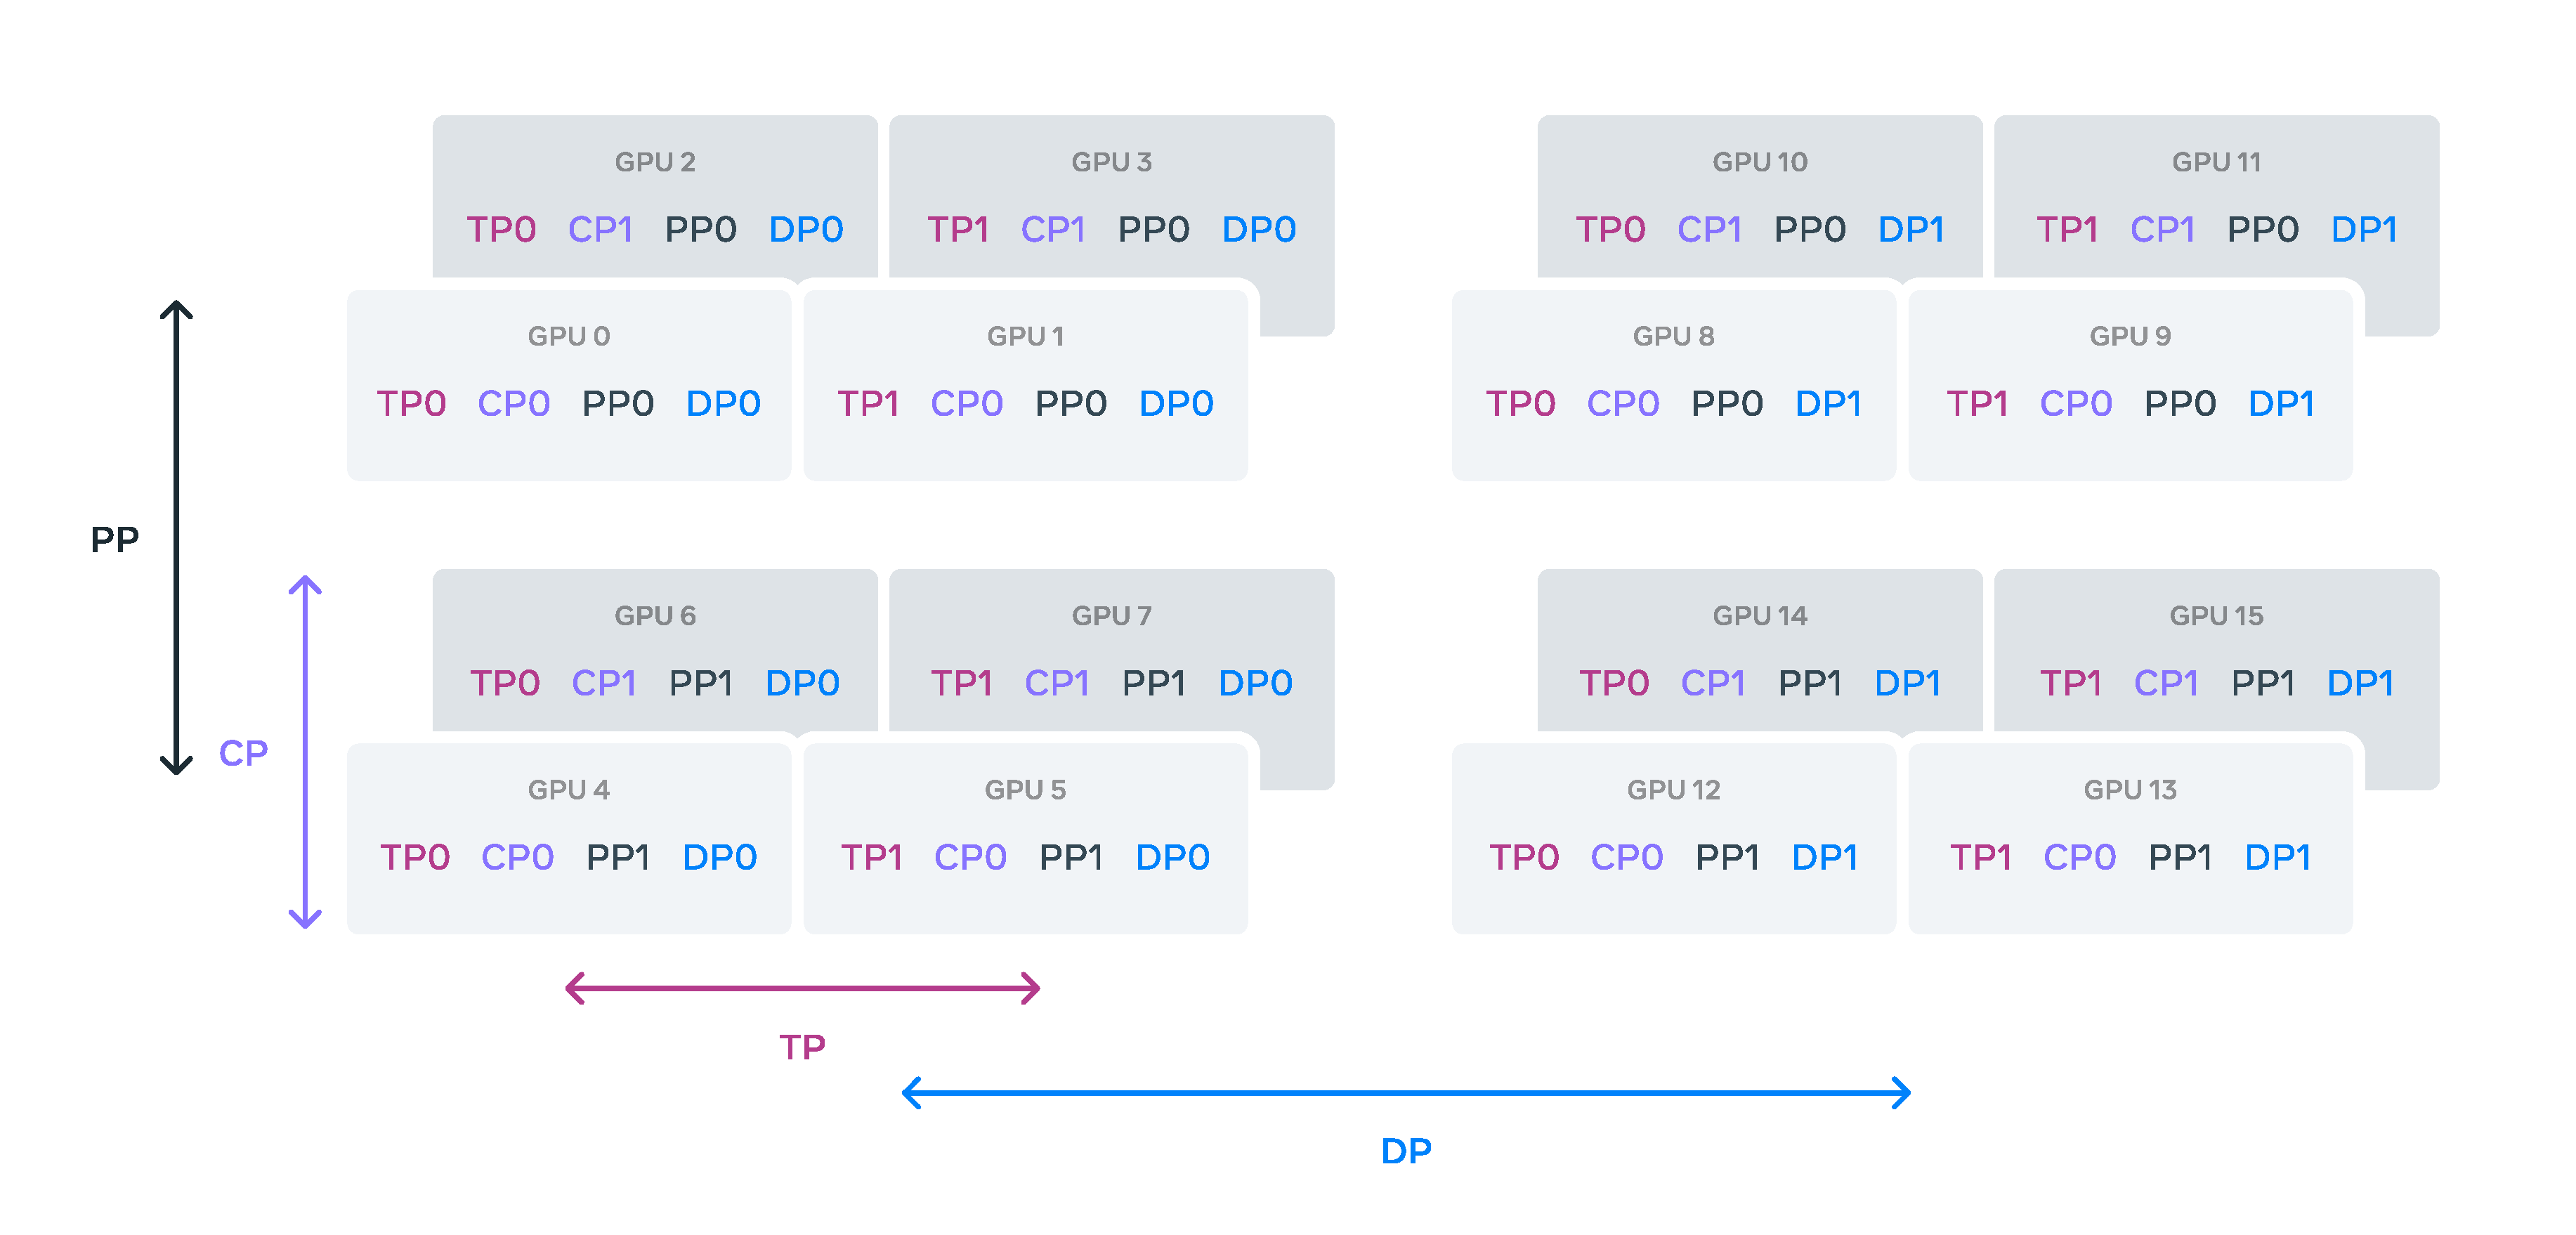
\includegraphics[width=\textwidth]{assets/4D_parallelism.pdf}
     \caption{\textbf{Illustration of 4D parallelism.} GPUs are divided into parallelism groups in the order of [TP, CP, PP, DP], where DP stands for FSDP. In this example, 16 GPUs are configured with a group size of |TP|=2, |CP|=2, |PP|=2, and |DP|=2. 
     A GPU's position in 4D parallelism is represented as a vector, [$D_1$, $D_2$, $D_3$, $D_4$], where $D_i$ is the index on the $i$-th parallelism dimension. In this example,
     GPU0[TP0, CP0, PP0, DP0] and GPU1[TP1, CP0, PP0, DP0] are in the same TP group, GPU0 and GPU2 are in the same CP group, GPU0 and GPU4 are in the same PP group, and GPU0 and GPU8 are in the same DP group.
     }
     \label{fig:4d_parallelism}
\end{figure}

\textbf{Pipeline parallelism improvements.}
We encountered several challenges with existing implementations:

\begin{itemize}
    \item \textbf{Batch size constraint.} Current implementations have constraints on supported batch size per GPU, requiring it to be divisible by the number of pipeline stages. For the example in Figure~\ref{fig:pipeline_parallelism}, the depth-first schedule (DFS) of pipeline parallelism~\citep{narayanan2021efficient} requires $N=\textrm{PP}=4$, while the breadth-first schedule (BFS; \citet{lamy2023breadth}) requires $N=M$, where $M$ is the total number of micro-batches and $N$ is the number of contiguous micro-batches for the same stage's forward or backward. However, pre-training often needs flexibility to adjust batch size.
    
    \item \textbf{Memory imbalance.} Existing pipeline parallelism implementations lead to imbalanced resource consumption. The first stage consumes more memory due to the embedding and the warm-up micro-batches.
    
    \item \textbf{Computation imbalance.} After the last layer of the model, we need to calculate output and loss, making this stage the execution latency bottleneck.
\end{itemize} 

To address these issues, we modify our pipeline schedule as shown in Figure~\ref{fig:pipeline_parallelism}, which allows setting $N$ flexibly---in this case $N=5$, which can run a arbitrary number of micro-batches in each batch. This allows us to run: (1) fewer micro-batches than the number of stages when we have batch size limit at large scale; or (2) more micro-batches to hide point-to-point communication, finding a sweet spot between DFS and breadth first schedule (BFS) for the best communication and memory efficiency. To balance the pipeline, we reduce one Transformer layer each from the first and the last stages, respectively. This means that the first model chunk on the first stage has only the embedding, and the last model chunk on the last stage has only output projection and loss calculation. To reduce pipeline bubbles, we use an interleaved schedule \citep{narayanan2021efficient} with $V$ pipeline stages on one pipeline rank. Overall pipeline bubble ratio is $\frac{\textrm{PP} - 1}{V * M}$. Further, we adopt asynchronous point-to-point communication in PP, which considerably speeds up training, especially in cases when the document mask introduces extra computation imbalance. We enable {\small \texttt{TORCH\_NCCL\_AVOID\_RECORD\_STREAMS}} to reduce memory usage from asynchronous point-to-point communication. Finally, to reduce memory cost, based on detailed memory allocation profiling, we proactively deallocate tensors that will not be used for future computation, including the input and output tensors of each pipeline stage, that will not be used for future computation. With these optimizations, we could pre-train \llamathree on sequences of 8K tokens without activation checkpointing.

\begin{figure*}[t]
     \centering
     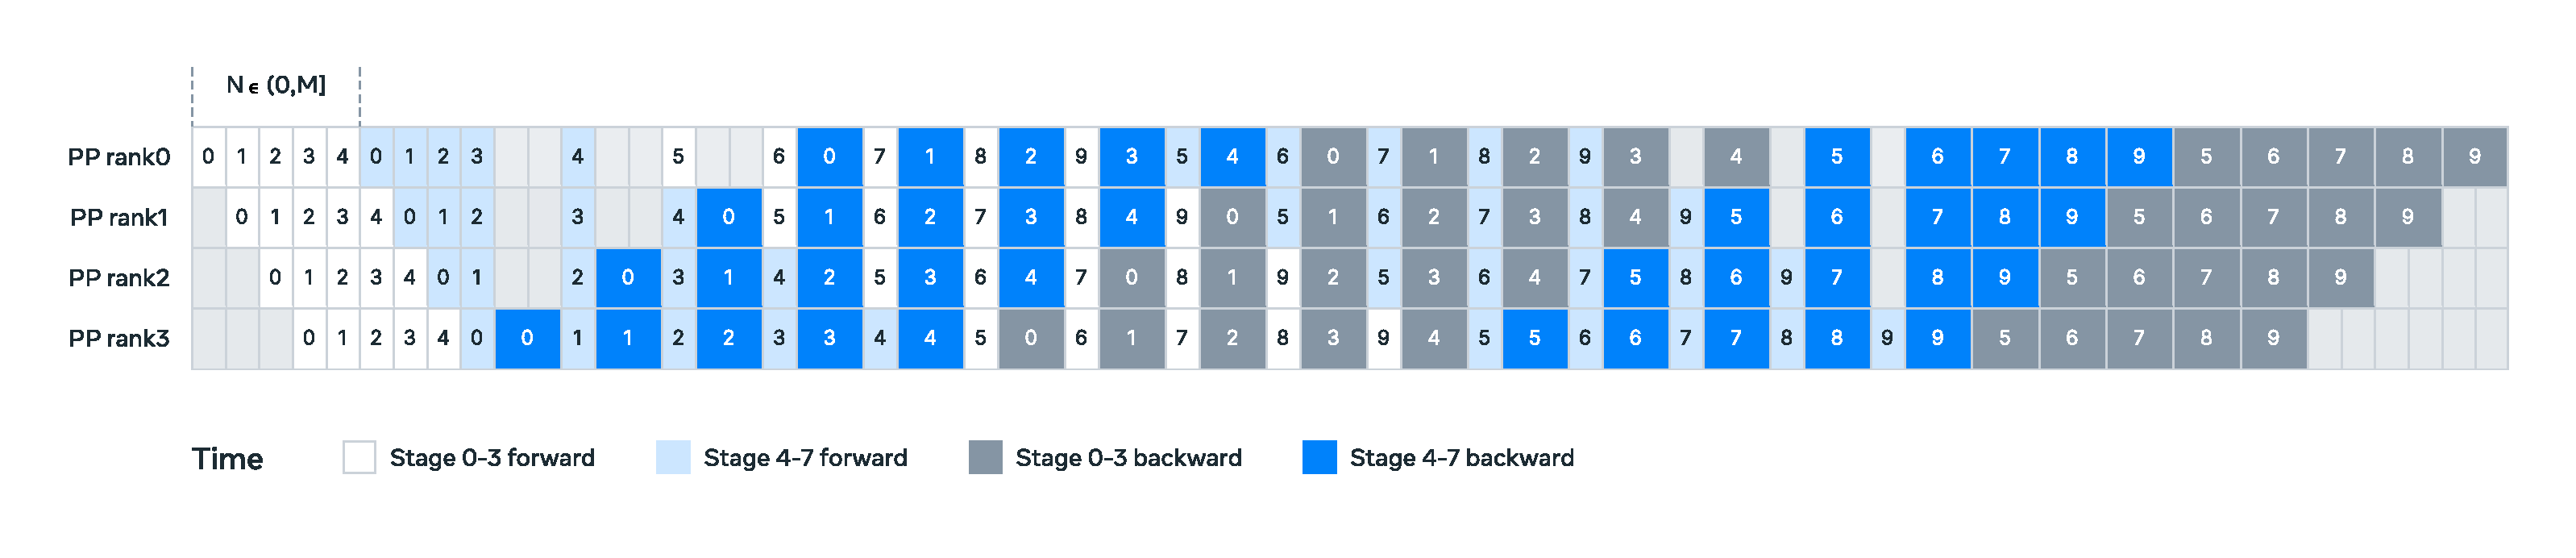
\includegraphics[width=\textwidth]{assets/pipeline_parallelism.pdf}
     \caption{\textbf{Illustration of pipeline parallelism in Llama 3.} Pipeline parallelism partitions eight pipeline stages (0 to 7) across four pipeline ranks (PP ranks 0 to 3), where the GPUs with rank 0 run stages 0 and 4, the GPUs with P rank 1 run stages 1 and 5, \emph{etc}. The colored blocks (0 to 9) represent a sequence of micro-batches, where $M$ is the total number of micro-batches and $N$ is the number of continuous micro-batches for the same stage's forward or backward. Our key insight is to make $N$ tunable.
     }
     \label{fig:pipeline_parallelism}
\end{figure*}

\textbf{Context parallelism for long sequences.} We utilize context parallelism (CP) to improve memory efficiency when scaling the context length of \llamathree and enable training on extremely long sequences up to 128K in length. In CP, we partition across the sequence dimension, and specifically we partition the input sequence into $2 \times \mbox{CP}$ chunks so each CP rank receives two chunks for better load balancing. The $i$-th CP rank received both the $i$-th and the $(2 \times \mbox{CP} - 1 - i)$-th chunks. 

Different from existing CP implementations that overlap communication and computation in a ring-like structure~\citep{liu2023ring}, our CP implementation adopts an \texttt{all-gather} based method where we first \texttt{all-gather} the key (K) and value (V) tensors, and then compute attention output for the local query (Q) tensor chunk. Although the \texttt{all-gather} communication latency is exposed in the critical path, we still adopt this approach for two main reasons: (1) it is easier and more flexible to support different types of attention masks in \texttt{all-gather} based CP attention, such as the document mask; and (2) the exposed \texttt{all-gather} latency is small as the communicated K and V tensors are much smaller than Q tensor due to the use of GQA \citep{ainslie2023gqa}. Hence, the time complexity of attention computation is an order of magnitude larger than \texttt{all-gather} ($O(S^2)$ versus $O(S)$, where $S$ represents the sequence length in the full causal mask), making the \texttt{all-gather} overhead negligible.

\textbf{Network-aware parallelism configuration.} The order of parallelism dimensions, [TP, CP, PP, DP], is optimized for network communication. The innermost parallelism requires the highest network bandwidth and lowest latency, and hence is usually constrained to within the same server. The outermost parallelism may spread across a multi-hop network and should tolerate higher network latency. Therefore, based on the requirements for network bandwidth and latency, we place parallelism dimensions in the order of [TP, CP, PP, DP]. DP (\emph{i.e.}, FSDP) is the outermost parallelism because it can tolerate longer network latency by asynchronously prefetching sharded model weights and reducing gradients. Identifying the optimal parallelism configuration with minimal communication overhead while avoiding GPU memory overflow is challenging. We develop a memory consumption estimator and a performance-projection tool which helped us explore various parallelism configurations and project overall training performance and identify memory gaps effectively.

\textbf{Numerical stability.} By comparing training loss between different parallelism setups, we fixed several numerical issues that impact training stability. To ensure training convergence, we use FP32 gradient accumulation during backward computation over multiple micro-batches and also \texttt{reduce-scatter} gradients in FP32 across data parallel workers in FSDP. For intermediate tensors, \emph{e.g.}, vision encoder outputs, that are used multiple times in the forward computation, the backward gradients are also accumulated in FP32.

\subsubsection{Collective Communication}
\label{sec:ncclx}

Our collective communication library for \llamathree is based on a fork of Nvidia's NCCL library, called NCCLX. NCCLX significantly improves the performance of NCCL, especially for higher latency networks. Recall that the order of parallelism dimensions is [TP, CP, PP, DP], where DP corresponds to FSDP. The outermost parallelism dimensions, PP and DP, may communicate through a multi-hop network, with latency up to tens of microseconds. The original NCCL collectives---\texttt{all-gather} and \texttt{reduce-scatter} in FSDP, and \texttt{point-to-point} in PP---require data chunking and staged data copy. This approach incurs several inefficiencies, including (1) requiring a large number of small control messages to be exchanged over the network to facilitate data transfer, (2) extra memory-copy operations, and (3) using extra GPU cycles for communication.  For \llamathree training, we address a subset of these inefficiencies by tuning chunking and data transfer to fit our network latencies, which can be as high as tens of microseconds for a large cluster. We also allow small control messages to traverse our network at a higher priority, especially avoiding being head-of-line blocked in deep-buffer core switches. Our ongoing work for future Llama versions involves making deeper changes in NCCLX to holistically address all the aforementioned problems.

\subsubsection{Reliability and Operational Challenges}

The complexity and potential failure scenarios of 16K GPU training surpass those of much larger CPU clusters that we have operated. Moreover, the synchronous nature of training makes it less fault-tolerant---a single GPU failure may require a restart of the entire job. Despite these challenges, for \llamathree, we achieved higher than 90\% effective training time while supporting automated cluster maintenance, such as firmware and Linux kernel upgrades~\citep{leonhardi2024maintenance}, which resulted in at least one~training interruption daily. The effective training time measures the time spent on useful training over the elapsed time.

During a 54-day snapshot period of pre-training, we experienced a total of 466 job interruptions. Of these, 47 were planned interruptions due to automated maintenance operations such as firmware upgrades or operator-initiated operations like configuration or dataset updates. The remaining 419 were unexpected interruptions, which are classified in Table~\ref{table:job_interruptions}.
Approximately 78\% of the unexpected interruptions are attributed to confirmed hardware issues, such as GPU or host component failures, or suspected hardware-related issues like silent data corruption and unplanned individual host maintenance events. GPU issues are the largest category, accounting for 58.7\% of all unexpected issues.  Despite the large number of failures, significant manual intervention was required only three times during this period, with the rest of issues handled by automation. 

\begin{table}[]
\centering
\begin{tabular}{lccc}
    \toprule
\textbf{Component}             & \textbf{Category} & \textbf{Interruption Count} & \textbf{\% of Interruptions} \\
\midrule
Faulty GPU                            & GPU               & 148                         & 30.1\%                       \\
GPU HBM3 Memory                & GPU               & 72                          & 17.2\%                       \\
Software Bug                   & Dependency          & 54                          & 12.9\%                       \\
Network Switch/Cable           & Network           & 35                          & 8.4\%                        \\
Host Maintenance               & \begin{tabular}[c]{@{}c@{}}Unplanned \\ Maintenance\end{tabular}       & 32                          & 7.6\%                        \\
GPU SRAM Memory                & GPU               & 19                          & 4.5\%                        \\
GPU System Processor           & GPU               & 17                          & 4.1\%                        \\
NIC                            & Host              & 7                           & 1.7\%                        \\
NCCL Watchdog Timeouts                  & Unknown           & 7                           & 1.7\%                        \\
Silent Data Corruption                      & GPU           & 6                           & 1.4\%                        \\
GPU Thermal Interface + Sensor & GPU               & 6                           & 1.4\%                        \\
SSD                            & Host              & 3                           & 0.7\%                        \\
Power Supply                   & Host              & 3                           & 0.7\%                        \\
Server Chassis                 & Host              & 2                           & 0.5\%                        \\
IO Expansion Board             & Host              & 2                           & 0.5\%                        \\
Dependency                     & Dependency        & 2                           & 0.5\%                        \\
CPU                            & Host              & 2                           & 0.5\%                        \\
System Memory                  & Host              & 2                           & 0.5\%    \\
\bottomrule
\end{tabular}
\caption{\textbf{Root-cause categorization of unexpected interruptions during a 54-day period of Llama 3 405B pre-training.} About 78\% of unexpected interruptions were attributed to confirmed or suspected hardware issues. }
\label{table:job_interruptions}
\end{table}

To increase the effective training time, we reduced job startup and checkpointing time, and developed tools for fast diagnosis and problem resolution. We extensively use PyTorch's built-in NCCL flight recorder~\citep{ansel2024pytorch}, a feature that captures collective metadata and stack traces into a ring buffer, and hence allowing us to diagnose hangs and performance issues quickly at scale, particularly with regard to NCCLX. Using this, we efficiently record every communication event and the duration of each collective operation, and also automatically dump tracing data on NCCLX watchdog or heartbeat timeout. We enable more computationally intensive tracing operations and metadata collection selectively as needed live in production through online configuration changes~\citep{configerator} without needing a code release or job restart.

Debugging issues in large-scale training is complicated by the mixed use of NVLink and RoCE in our network. Data transfer over NVLink typically occurs through load/store operations issued by CUDA kernels, and failures in either the remote GPU or NVLink connectivity often manifest as stalled load/store operations within CUDA kernels without returning a clear error code. NCCLX enhances the speed and accuracy of failure detection and localization through a tight co-design with PyTorch, allowing PyTorch to access NCCLX’s internal state and track relevant information. While stalls due to NVLink failures cannot be completely prevented, our system monitors the state of the communication library and automatically times out when such a stall is detected. Additionally, NCCLX traces the kernel and network activities of each NCCLX communication and provides a snapshot of the failing NCCLX collective's internal state, including finished and pending data transfers between all ranks. We analyze this data to debug NCCLX scaling issues.

Sometimes, hardware issues may cause still-functioning but slow stragglers that are hard to detect. Even a single straggler can slow down thousands of other GPUs, often appearing as functioning but slow communications. We developed tools to prioritize potentially problematic communications from selected process groups. By investigating just a few top suspects,  we were usually able to effectively identify the stragglers.

One interesting observation is the impact of environmental factors on training performance at scale. For Llama 3 405B , we noted a diurnal 1-2\% throughput variation based on time-of-day. This fluctuation is the result of higher mid-day temperatures impacting GPU dynamic voltage and frequency scaling.

During training, tens of thousands of GPUs may increase or decrease power consumption at the same time, for example, due to all GPUs waiting for checkpointing or collective communications to finish, or the startup or shutdown of the entire training job. When this happens, it can result in instant fluctuations of power consumption across the data center on the order of tens of megawatts, stretching the limits of the power grid. This is an ongoing challenge for us as we scale training for future, even larger Llama models.
